\section{Theoretical overview}
\label{sec:theory}

\subsection{The Standard Model of Particle Physics}

The Standard Model (SM) of particle physics is a collection of theories incorporating quantum electrodynamics, quantum chromodynamics and the Glashow-Weinberg-Salam theory of the electroweak interaction. It describes our current understanding of elementary particles and their interactions. While this section briefly describes the most relevant aspects of the SM for this thesis, a more complete description can be found in~\cite{griffiths,halzen}.

\subsubsection{Constituents of the SM}

The elementary particles in the SM can be divided into two categories: fermions, with half integer spin, and bosons, with integer spin. The SM fermions consist of quarks and leptons and form the building blocks of nature. The bosons mediate the fundamental interactions between the fermions. In the SM, this corresponds to the electromagnetic, the strong and the weak forces. The properties of each of these bosons are shown in Table~\ref{tab:bosons}. Gravity, the weakest of the four fundamental forces, is not included in the SM.

\begin{table}[!b]
\caption{The fundamental interactions of the SM, their corresponding bosons and their typical coupling.}
\begin{center}
\begin{tabular}{lll}
Force & Boson & Typical coupling $\alpha_{i}$ \\
\hline
Strong & $g$ & 1 \\
Electromagnetic & \g & 10$^{-2}$ \\
Weak &  \Z, \Wpm & 10$^{-6}$ \\
\end{tabular}
\end{center}
\label{tab:bosons}
\end{table}

Quarks and leptons are grouped into three generations of increasing mass
\begin{equation}
{\rm quarks}: \binom{\uquark}{\dquark},~\binom{\cquark}{\squark},~\binom{\tquark}{\bquark} ~~~ {\rm leptons}: \binom{\neue}{\electron},~\binom{\neum}{\mu},~\binom{\neut}{\tau}. \nonumber
\end{equation}  
\noindent Quarks come in six `flavours': up, down, charm, strange, top and bottom. For leptons, each generation contains a charged lepton and a neutrino. There are three different flavours of lepton: electron, muon and tau. The properties of each of the SM fermions are shown in Table~\ref{tab:fermions}. Each fermion has a corresponding antiparticle with equal mass and lifetime but opposite charge and internal quantum numbers.

\begin{table}[!tb]
\def\arraystretch{1.1}
\caption{Properties of the quarks and leptons in the SM. The particle masses are taken from~\cite{pdg}.}
\begin{center}
\resizebox{\textwidth}{!}{
\begin{tabular}{ccc}
\multicolumn{3}{c}{\bf Quarks} \\
Flavour & Mass~[\mevcc] & Charge \\
\hline
\uquark & $2.3^{+0.7}_{-0.5}$ & $+$2/3 \\
\dquark & $4.8^{+0.7}_{-0.3}$ & $-$1/3 \\
\cquark & $1275\pm25$ & $+$2/3 \\
\squark & $95\pm5$ & $-$1/3 \\
\tquark & $(160^{+5}_{-4})\times10^{3}$ & $+$2/3 \\
\bquark & $4180\pm30$ & $-$1/3 \\
\end{tabular}

\begin{tabular}{ccc}
\multicolumn{3}{c}{\bf Leptons} \\
Flavour & Mass~[\mevcc] & Charge \\
\hline
\neue & $<2 \times 10^{-6}$ & \hphantom{$-$}0 \\
\electron & 0.510998928(11) & $-$1 \\
\neum & $<0.19$ & \hphantom{$-$}0 \\
\muon & 105.6583715(35) & $-$1 \\
\neut & $<18.2$ & \hphantom{$-$}0 \\
\tauon & 1776.86(12) & $-$1 \\
\end{tabular}
}
\end{center}
\label{tab:fermions}
\end{table}

The electromagnetic force is mediated by the photon, and acts on all charged particles. As photons are electrically neutral they do not interact with each other.

Quarks carry a type of charge called `colour' which comes in three types: red, green and blue. As such, they are able to participate in the strong interaction, which is also referred to as quantum chromodynamics (QCD). Antiquarks carry anticolour (antired, antiblue, antigreen), while gluons are bicoloured and carry one positive unit of colour and one negative unit. Therefore, a quark can change colour by exchanging a gluon with another quark. Unlike photons, gluons can undergo self interaction. 

As QCD only allows colourless objects, quarks are confined within bound states called hadrons. There are two types of hadrons: baryons, containing three quarks each with a different colour, and mesons, containing a quark and an antiquark with opposite colour. The main focus of this thesis is the study of \B mesons which contain either a \bquark quark or a \bquarkbar quark.

The weak force is mediated by the massive \Wpm and \Z bosons and acts on all fermions. Like the electromagnetic and strong interactions the neutral weak current, which involves the exchange of a \Z boson, is flavour conserving. However, the charged weak current, which involves the exchange of a \Wpm boson, changes the flavour of a quark from an up-type to a down-type and vice versa.

The Higgs boson, \H, is a scalar particle that results from the mechanism of electroweak symmetry breaking, through which the \Wpm and \Z are given a mass due to the non zero vacuum expectation value of the Higgs field. It was the final particle of the SM to be discovered when it was confirmed in 2012~\cite{higgs-atlas,higgs-cms}. The quarks and leptons also obtain their masses via interactions with the Higgs field. 

\subsubsection{Flavour violation in the SM}

When only the three lightest quarks (\uquark, \dquark, \squark) were known, Cabibbo~\cite{cabbibo} proposed a mechanism to explain the observed rates of semileptonic processes. Vertices of the type $\decay{\dquark}{\uquark+\Wm}$ were given a factor $\cos\theta_{C}$, while those of the type $\decay{\squark}{\uquark+\Wm}$ were given a factor $\sin\theta_{C}$, where $\theta_{C}\sim13^{\circ}$ is the Cabibbo angle. This mechanism was found to be very successful in describing many decay rates but there was a problem: it allowed the \Kz meson to decay into a \mumu pair. The amplitude of this process should be proportional to $\sin\theta_{C}\cos\theta_{C}$ but the calculated rate was much greater than the experimental limit. 

A solution was proposed by Glashow, Iliopoulos and Maini (GIM)~\cite{gim} who introduced the fourth quark, \cquark, with vertex couplings of $-\sin\theta_{C}$ and $\cos\theta_{C}$ for $\decay{\dquark}{\cquark+\Wm}$ and $\decay{\squark}{\cquark+\Wm}$ transitions respectively. This was several years before the \cquark quark was observed experimentally~\cite{jpsi-1,jpsi-2}. According to the GIM mechanism, the diagram for the decay \decay{\Kz}{\mumu} in Fig.~\ref{fig:ktomm:a} is almost exactly cancelled by the corresponding diagram in Fig.~\ref{fig:ktomm:b} with a virtual \cquark quark replacing the \uquark. The small rate that remains is due to the differences in the masses of the \uquark quark and the \cquark quark.

\begin{figure}[!tb]
\centering
\begin{subfigure}{0.49\textwidth}
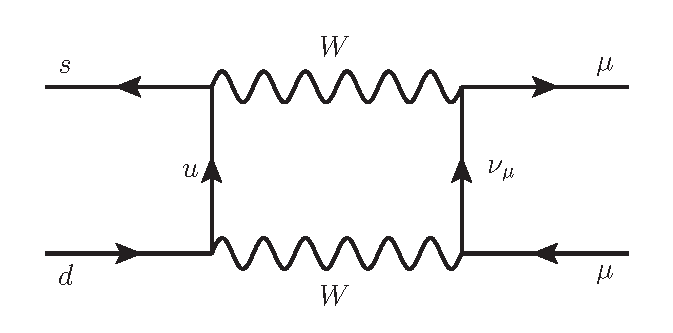
\includegraphics[width=\linewidth]{figs/theory/KToMuMu_uquark.eps}
\caption{}
\label{fig:ktomm:a}
\end{subfigure}
\begin{subfigure}{0.49\textwidth}
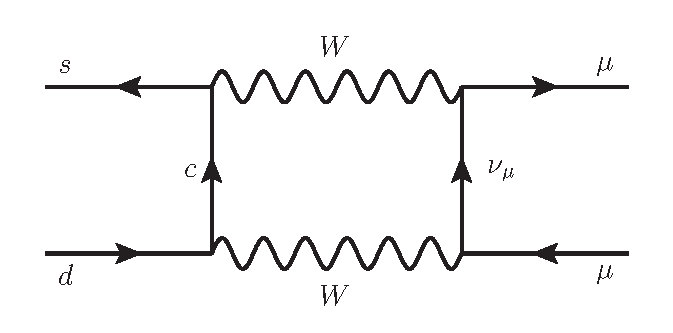
\includegraphics[width=\linewidth]{figs/theory/KToMuMu_cquark.eps}
\caption{}
\label{fig:ktomm:b}
\end{subfigure}
\caption{Feynman diagrams contributing to the decay \decay{\Kz}{\mumu}. The amplitude for each diagram is proportional to the product of the coupling at each vertex: (a) $\sin\theta_{C}\cos\theta_{C}$, (b)  $-\sin\theta_{C}\cos\theta_{C}$. The total amplitude is found by summing the two contributions.}
\label{fig:ktomm}
\end{figure}

In the Cabibbo-GIM scheme, it can be intepreted that the \W does not couple to the mass eigenstates \dquark and \squark but instead to the weak eigenstates $\dquark^\prime$ and $\squark^\prime$, given by

\begin{equation}
\dquark^\prime = \dquark\cos\theta_{C}+\squark\sin\theta_{C},~~~\squark^\prime = -\dquark\sin\theta_{C}+\squark\cos\theta_{C}
\end{equation}

\noindent or in `Cabibbo matrix' form

\begin{equation}
\binom{\dquark^\prime}{\squark^\prime} = 
\begin{pmatrix}
\cos\theta_{C} & \sin\theta_{C} \\
-\sin\theta_{C} & \cos\theta_{C} \\
\end{pmatrix}
\binom{\dquark}{\squark}.
\end{equation}

Even before the discovery of the \cquark quark, Kobayaski and Maskawa~\cite{kobayashi-maskawa} had generalised the Cabibbo-GIM scheme to incorporate three generations of quarks. This was motivated by the desire to explain \CP violation within the Cabibbo-GIM scheme, which was not possible with only two generations. The weak eigenstates are related to the mass eigenstates through the CKM matrix

\begin{equation}
\begin{pmatrix}
\dquark^\prime \\
\squark^\prime \\
\bquark^\prime \\
\end{pmatrix}
=
\begin{pmatrix}
\Vud & \Vus & \Vub \\
\Vcd & \Vcs & \Vcb \\
\Vtd & \Vts & \Vtb \\
\end{pmatrix}
\begin{pmatrix}
\dquark \\
\squark \\
\bquark \\
\end{pmatrix}
\end{equation}

\noindent where each matrix element, \Vij, specifies the coupling of $i$ to $j$. The additional generation of quarks increases the number of free parameters from one ($\theta_{C}$) to four: three `generalised Cabibbo angles' ($\theta_{12}$, $\theta_{23}$, $\theta_{13}$) and a complex phase $\delta$. This complex phase is the dominant source of \CP violation in the SM. 

\subsection{Beyond the SM}

Despite the considerable success of the SM it is not without its limitations, some of which are outlined below

\begin{itemize}
  \item Gravity, the fourth fundamental force, is not incorporated in the SM.
  \item The SM has a large number of free parameters many of which relate to the flavour sector: the 9 fermion masses, the four parameters of the CKM matrix and a \CP violating phase in the strong sector.
  \item Dark matter and dark energy, which make up 95\% of the mass of the Universe, are not accounted for in the SM.
  \item The amount of \CP violation predicted by the SM is ten orders of magnitude lower than what is needed to account for the observed matter-antimatter asymmetry in the Universe.
\end{itemize}

\noindent These limitations have led physicists to look for extensions to the SM in the form of New Physics (NP) models. Such NP models often predict new particles that may contribute to, and therefore modify, flavour-changing processes in the SM.

\subsection{Rare decays of \B mesons}

Flavour-changing neutral current (FCNC) transistions are forbidden at tree level in the SM. They are rare processes that occur at loop level, making them an ideal place to perform a search for NP. Rare decays of \B mesons, such as those containing a \btosll transition, can have sizeable NP contributions that are not swamped by the competing SM process. 

By studying the properties of FCNC processes it is possible to perform model independent searches sensitive to a wide range of NP models. Feyman diagrams for the \btosll transition, both in the SM and in proposed NP models~\cite{bstoll-higgs,bstoll-zprime}, are shown Fig.~\ref{fig:btosll}. New particles can modify the dynamics of a decay: changing the branching fraction or the kinematic distribution of the final state particles. By comparing the SM prediction of observables with experimental measurements, the flavour structure of NP models can be probed. The theoretical framework in which flavour physics measurements are intepreted is known as Operator Product Expansion (OPE)~\cite{ope}.

\begin{figure}[!tb]
\centering
\begin{subfigure}{0.49\textwidth}
\begin{tikzpicture}
\node[anchor=south west,inner sep=0](image) at (0,0) {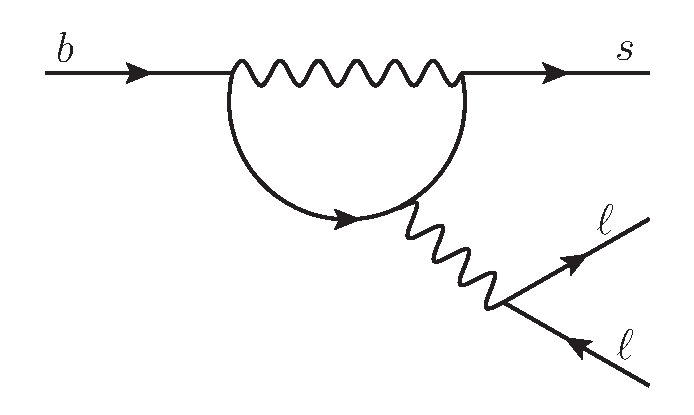
\includegraphics[width=\textwidth]{figs/theory/btosll_penguin.eps}};
\begin{scope}[x={(image.south east)},y={(image.north west)}]
%\draw[help lines,xstep=.1,ystep=.1] (0,0) grid (1,1);
\node[draw=none,bleudefrance] at (0.53,0.96) {\small \Wm};
\node[draw=none,bleudefrance] at (0.3,0.6) {\small \tquark};
\node[draw=none,bleudefrance] at (0.56,0.27) {\small \Pgamma, $\Z^{0}$};
\node[draw=none,bleudefrance] at (0.2,0.2) {SM};
\end{scope}
\end{tikzpicture}
\caption{}
\label{fig:btosll:a}
\end{subfigure}
\begin{subfigure}{0.49\textwidth}
\begin{tikzpicture}
\node[anchor=south west,inner sep=0](image) at (0,0) {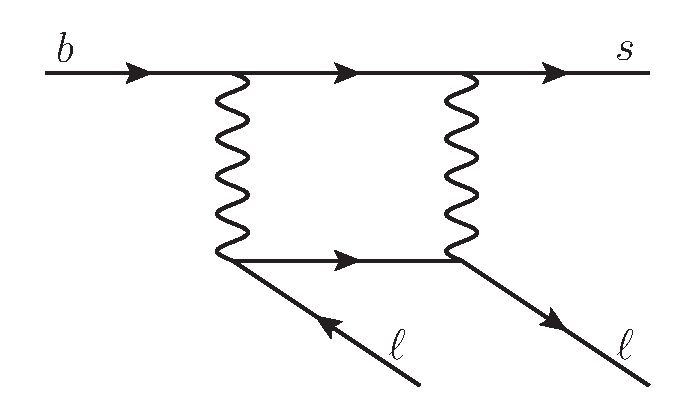
\includegraphics[width=\textwidth]{figs/theory/btosll_box.eps}};
\begin{scope}[x={(image.south east)},y={(image.north west)}]
%\draw[help lines,xstep=.1,ystep=.1] (0,0) grid (1,1);
\node[draw=none,bleudefrance] at (0.5,0.95) {\small \tquark};
\node[draw=none,bleudefrance] at (0.25,0.6) {\small \Wm};
\node[draw=none,bleudefrance] at (0.8,0.6) {\small \Wp};
\node[draw=none,bleudefrance] at (0.5,0.45) {\small \Pnu};
\node[draw=none,bleudefrance] at (0.2,0.2) {SM};
\end{scope}
\end{tikzpicture}
\caption{}
\label{fig:btosll:b}
\end{subfigure}
\begin{subfigure}{0.49\textwidth}
\begin{tikzpicture}
\node[anchor=south west,inner sep=0](image) at (0,0) {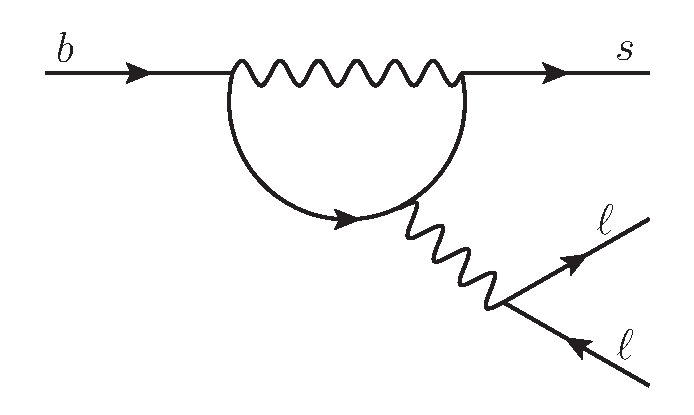
\includegraphics[width=\textwidth]{figs/theory/btosll_penguin.eps}};
\begin{scope}[x={(image.south east)},y={(image.north west)}]
%\draw[help lines,xstep=.1,ystep=.1] (0,0) grid (1,1);
\node[draw=none,bostonuniversityred] at (0.5,0.96) {\small $\tilde{g}$};
\node[draw=none,bostonuniversityred] at (0.3,0.6) {\small $\tilde{d}_{i}$};
\node[draw=none,bostonuniversityred] at (0.58,0.27) {\small $\H$};
\node[draw=none,bostonuniversityred] at (0.2,0.2) {NP};
\end{scope}
\end{tikzpicture}
\caption{}
\label{fig:btosll:c}
\end{subfigure}
\begin{subfigure}{0.49\textwidth}
\begin{tikzpicture}
\node[anchor=south west,inner sep=0](image) at (0,0) {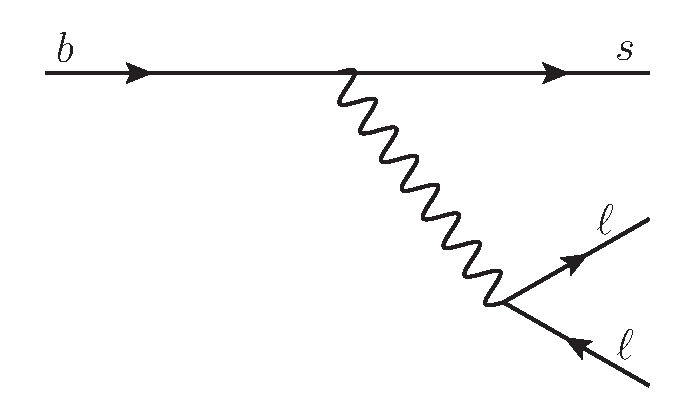
\includegraphics[width=\textwidth]{figs/theory/btosll_zprime.eps}};
\begin{scope}[x={(image.south east)},y={(image.north west)}]
%\draw[help lines,xstep=.1,ystep=.1] (0,0) grid (1,1);
\node[draw=none,bostonuniversityred] at (0.55,0.45) {\small $Z^{'}$};
\node[draw=none,bostonuniversityred] at (0.2,0.2) {NP};
\end{scope}
\end{tikzpicture}
\caption{}
\label{fig:btosll:d}
\end{subfigure}
\caption{Feynman diagrams for the FCNC transition \btosll: in the SM (a,b) and in possible NP scenarios (c,d).}
\label{fig:btosll}
\end{figure}

In the OPE approach, all degrees of freedom above a given energy scale, $\Lambda$, are integrated out. This is valid as long as $\Lambda$ is much larger than the energy scale of the decay, $\mu$, which for the study of \B mesons is chosen to be $\order(m_{\bquark})$. This formalism is analogous to Fermi's effective theory of weak decay in which the full theory is reduced to a four point interaction, as shown in Fig.~\ref{fig:beta} for $\beta$-decay.

\begin{figure}[!tb]
\centering
\begin{subfigure}{0.49\textwidth}
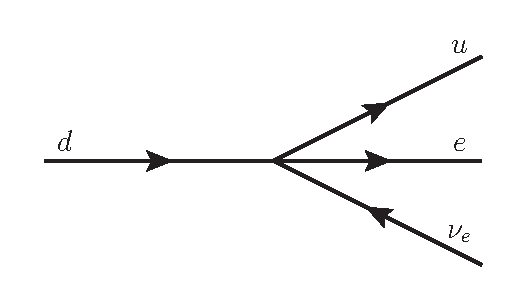
\includegraphics[width=\linewidth]{figs/theory/beta_4point.eps}
\caption{}
\label{fig:beta:a}
\end{subfigure}
\begin{subfigure}{0.49\textwidth}
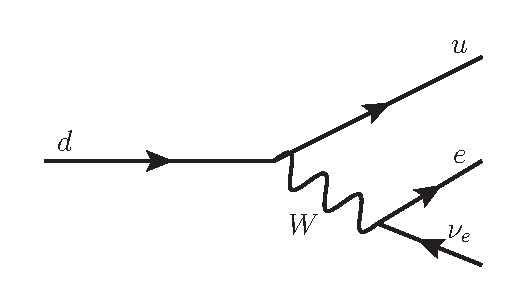
\includegraphics[width=\linewidth]{figs/theory/beta_w.eps}
\caption{} 
\label{fig:beta:b}
\end{subfigure}
\caption{Feynman diagrams for $\beta$-decay in the (a) effective theory and (b) full theory.}
\label{fig:beta}
\end{figure}

In the SM, the effective Hamiltonian describing \btosll decays can be written as

\begin{equation}
\mathcal{H}_{\rm eff} = - \frac{4G_{F}}{\sqrt{2}}V_{tb}V^{*}_{ts}\sum_{i}[\mathcal{C}_{i}(\mu)\mathcal{O}_{i}(\mu) + \mathcal{C}^{'}_{i}(\mu)\mathcal{O}^{'}_{i}(\mu)].
\end{equation}

\noindent where $G_{F}$ is the Fermi constant, and $V_{ij}$ are CKM matrix elements. The complex Wilson coefficients, $\mathcal{C}_{i}$, incorporate the short distance (high energy) contributions. For each Wilson coefficient, there is a local operator $\mathcal{O}_{i}$ which incorporates the long distance (low energy) contributions. The primed operators represent the right-handed currents, which are highly suppressed in the SM. The advantage of the OPE approach is that the Wilson coefficients are independent of the underlying process and can include contributions from NP contributions. 

For \btosll decays, the dominant contributions in the SM arise from the following operators~\cite{operators}

\begin{alignat}{2}
&\order_{7} = \frac{e}{g^{2}}m_{\bquark}(\squarkbar\sigma_{\mu\nu}P_{R}\bquark)F^{\mu\nu},~~~~~&&\order_{7}^{\prime} = \frac{e}{g^{2}}m_{\bquark}(\squarkbar\sigma_{\mu\nu}P_{L}\bquark)F^{\mu\nu}, \nonumber \\
&\order_{9} = \frac{e^{2}}{g^{2}}(\squarkbar\gamma_{\mu}P_{L}\bquark)(\ellbar\gamma^{\mu}\ell), &&\order_{9}^{\prime} = \frac{e^{2}}{g^{2}}(\squarkbar\gamma_{\mu}P_{R}\bquark)(\ellbar\gamma^{\mu}\ell),\\
&\order_{10} = \frac{e^{2}}{g^{2}}(\squarkbar\gamma_{\mu}P_{L}\bquark)(\ellbar\gamma^{\mu}\gamma_{5}\ell), &&\order_{10}^{\prime} = \frac{e^{2}}{g^{2}}(\squarkbar\gamma_{\mu}P_{R}\bquark)(\ellbar\gamma^{\mu}\gamma_{5}\ell), \nonumber
\end{alignat}

\noindent where $P_{L/R} = (1\mp\gamma_{5})/2$ are the left- and right-handed projection operators. The operator $\order_{7}$ is the electromagnetic operator corresponding to the emission of a photon. The vector and axial-vector operators, $\order_{9}$ and $\order_{10}$, describe the $Z$ penguin and $W$ box diagrams.

